%%%%%%%%%%%%%%%%%%%%%%%%%%%%%%%%%%%%%%%%%%%%%%%%%%%%%%%%%%%%%%%%%%%%%%%%%%%%%%%%
% experiment.tex: Chapter describing the experiment
%%%%%%%%%%%%%%%%%%%%%%%%%%%%%%%%%%%%%%%%%%%%%%%%%%%%%%%%%%%%%%%%%%%%%%%%%%%%%%%%
\chapter{Experiment}
\label{experiment_chapter}
%%%%%%%%%%%%%%%%%%%%%%%%%%%%%%%%%%%%%%%%%%%%%%%%%%%%%%%%%%%%%%%%%%%%%%%%%%%%%%%%
%\subsection{Overview of the Compact Muon Solenoid and Large Hadron Collider}
The Compact Muon Solenoid (CMS) experiment was built to detect all Standard Model (SM) particles, and to
search for any non-SM interactions that produce SM particles, such as the interaction described in 
chapter ~\ref{sec:wrBosonAndHeavyNu}.  Two high-energy proton beams collided at the geometric center of
the CMS experiment, and interactions between colliding protons were recorded.

Interactions between protons were identified by the detection of one or more of the following events:
\begin{itemize}
	\item trigger description, followed by particle flow event reconstruction
\end{itemize}


The Compact Muon Solenoid (CMS) was built to detect new particles produced by proton-proton (pp) collisions 
in the Large Hadron Collider (LHC).  Situated underground near the French-Swiss border and
operated by the European Organization for Nuclear Research (CERN), the LHC collided protons at
$\sqrt{s} = 13\TeV$ center-of-mass energy to search for new particles like the \WR boson discussed 
in Sec. ~\ref{sec:wrBosonAndHeavyNu}.  Evidence of the \WR boson was sought in pp collision events that
produced Standard Model (SM) leptons and hadronic jets.  The CMS detector used to identify leptons and
jets is described herein.

The

%use this lumi info in the trigger section.  it is not relevant for the detection of leptons and jets
%why are high lumi and energy needed
The LHC was built to discover new physics mediated by heavy particles which are weakly coupled to Standard Model (SM)
leptons, hadrons and bosons.  To produce heavy, weakly interacting particles, like a $2.0 TeV$ mass right handed W ($W_{R}$) boson
with production cross section 5 fb, at a rate sufficient for detection, average instantaneous luminosities of
$10^{33} \frac{1}{cm^{2}s}$ are needed.  At such luminosities, other more abundant or lower energy processes will occur
at a significant rate, as shown in Figure \ref{fig:smProductionXsxns}.

Of all processes created by collisions in the LHC, low energy, inelastic QCD interactions occur at the highest rate, of the order
$10^{8}$ events per second at $10^{33} \frac{1}{cm^{2}s}$.  Contributions from these events to new physics searches are mitigated by vetoing
on large groups of particles collinear with the beam line, or requiring the presence of leptons or photons.  However, these
requirements are not sufficient to suppress leptonic backgrounds created by the production and decay of heavy quarks, and QCD multijet
events in which a jet is incorrectly reconstructed as a lepton due to energetic neutral pions in the jet.  Such high energy QCD multijet
and heavy quark decay events occur at a rate of $10^{5}$ events per second at $10^{33} \frac{1}{cm^{2}s}$.  These event rates dwarf
the rate at which entire events can be read out of CMS and saved to disk, approximately $10^{3}$ events per second.  The tools, generally
called triggers, used to select and save collision events at approximately $10^{3}$ Hz will be discussed later.

\begin{figure}[h]
	\centering
	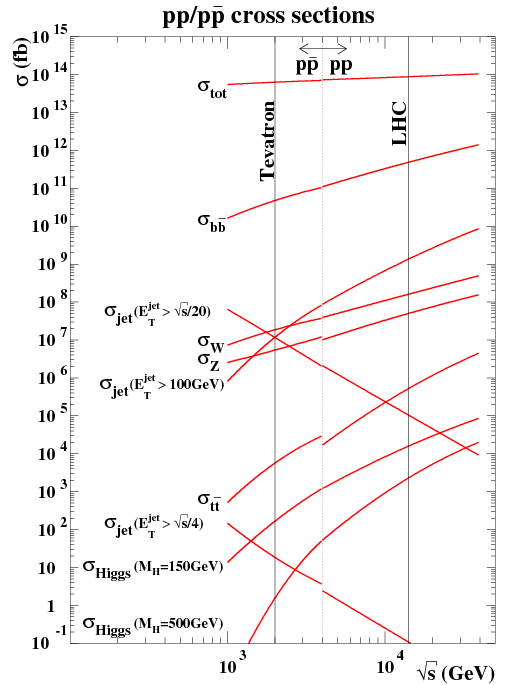
\includegraphics[width=0.6\textwidth]{figures/lhc_and_tevatron_cross_sections_2006.png}
	\caption{Production cross sections at the LHC and Tevatron as a function of center of mass energy. \cite{}}
	\label{fig:smProductionXsxns}
\end{figure}


%Operations
The LHC started operations with collisions at a lower center of mass energy and lower instantaneous luminosity than design.  In 2015 the center of mass
energy was increased to 13 TeV, and the luminosity was increased closer to the design level.  The 2015 data taking period was split into two portions - from the start
of 2015 collisions until August the time separation between consecutive proton bunches in each beam was 50 ns.  After August, the bunch
separation decreased to 25 ns to increase the instantaneous luminosity, and proton proton collisions continued until November.  From August until November, instantaneous 
luminosities reached $5x10^{33} \frac{1}{cm^{2}s}$, but problems with the CMS
magnet cooling system limited the amount of data collected to 2.6 $fb^{-1}$.  Decreasing the bunch spacing increased the sensitivity of every new physics search, but
came with the cost of more proton proton interactions in every bunch collision, or pileup.  At 13 TeV the total inelastic cross section is approximately 70 mb \cite{Haevermaet}, 
so for instantaneous luminosities between $3-5x10^{33} \frac{1}{cm^{2}s}$ in 25 ns running the expected pileup per bunch crossing is $8-13$, which is consistent with
the pileup observed in 25 ns collision data.  Pileup increases the complexity of events$\footnote{15 inelastic pp collisions yield a total flux of particles similar to one top antitop quark pair event}$, and makes event reconstruction and offline analysis more challenging.


\subsection{Compact Muon Solenoid Detector Overview}
\begin{itemize}
	\item trigger description, followed by particle flow event reconstruction
\end{itemize}
The Compact Muon Solenoid (CMS) experiment is designed to search for signs of new physics at the high energy and luminosity regime probed by the LHC.  The LHC was built
as a discovery machine, so particular attention has been paid to searches for physics beyond the SM (BSM), such as supersymmetry and extensions of the SM.

The The CMS detector approximates a cylinder in shape, with a length of 22 meters, outer radius of 7 meters, and weight of 14500 tons.  It is divided into a central barrel region ($|\eta| < 1.4$)
in which separate subdetectors are arranged as concentric cylindrical shells at increasing radii from the beam axis, and a forward endcap region ($|\eta| > 1.4$) 
in which subdetectors are arranged as layers stacked along the beam axis.  Illustrated in Figure \ref{fig:cmsDetectorComponentView}, the CMS subdetectors have complete 2$\pi$ radian coverage in
$\phi$, and hermetic calorimeter coverage from $-5 \leq \eta \leq 5$ ($-179^{\circ} \leq \theta \leq 0.77^{\circ}$) with respect to the beam axis.  Complete detector
coverage over this large angular range allows precise measurements to be made of missing energy, and the mass of yet-undiscovered light and heavy particles.

\begin{figure}[h]
	\centering
	
\includegraphics[width=0.6\textwidth]{figures/missingImage.png}
	\caption{The CMS detector with the coordinate system shown   .  The x axis points towards...}
	\label{fig:cmsDetectorComponentView}
\end{figure}


Starting at the interaction point and going radially outward, the first subdetector encountered by particles produced in collisions is the silicon tracker.
The tracker consists of silicon pixel detectors surrounded by silicon strip detectors, all of which are immersed in a 3.8 Tesla magnetic field produced by a superconducting solenoid.
Both detectors are only sensitive to charged particles, and facilitate precise measurements of charged particle momenta
and the positions of interaction vertices by measuring the curvature of charged particle tracks which have $|\eta| \leq 2.5$.

Particles which exit the tracker with sufficient momentum to travel approximately 1.0 meter radially away from the interaction point will reach the
electromagnetic calorimeter (ECAL).  ECAL consists of approximately 76000 lead tungstate crystals which, like the tracker, are sit in a 3.8 Tesla
magnetic field.  The radiation hardness and fast scintillation time of lead tungstate were key factors in chosing to build ECAL out of it.
ECAL was designed to measure the energy, time, position and shower shape of electrons and photons with $|\eta| \leq 3.0$ by measuring scintillation
light produced by lead tungstate in electron and photon showers.

Particles which traverse ECAL with sufficient momentum to continue moving away from the interaction point hit the hadronic calorimeter (HCAL).  Built
from alternating layers of metal and scintillating plastic tiles, HCAL was designed to measure the energy of charged and neutral
hadrons, and to provide structural support to all of CMS.  Energetic hadrons produce showers of lower energy particles in metal layers, and the
showers which reach nearby scintillating tiles produce scintillation light.
HCAL extends out to $|\eta| = 3.0$, is enveloped by the 3.8 Tesla magnetic field, and
is complimented by a forward hadron calorimeter (HF) which extends the calorimetry coverage out to $|\eta| = 5.0$.  Due to the high radiation
environment in its vicinity, HF is built from radiation hard steel blocks laced with radiation hard quartz fibers.  Charged particles which travel
through HF produce Cherenkov light in the quartz fibers; from the Cherenkov light an energy measurement is extracted.

Surrounding HCAL is the CMS magnet.  It produces a 3.8 Tesla magnetic field from superconducting niobium titanate wire wound into a solenoid, and
carries more than 10000 amps of current during normal operation.

Particles which pass through HCAL and the magnet encounter the last CMS subdetector, designed to measure the energy of muons.  The muon
detectors consist of three technologies - drift tubes (DT) and resistive plate chambers (RPC) which cover out to $|\eta| \leq 1.3$, while cathode
strip chambers (CSC) and RPCs which cover $1.3 \leq |\eta| \leq 2.4$, with some overlap near $|\eta| = 1.3$.  All three technologies measure the amount
of charge ionized in a gas when a muon traverses an enclosed volume filled with gas, and convert this charge into an energy.

All CMS subdetectors are utilized in particle flow (PF) reconstruction and event triggering.  In. 

\subsection{Track and vertex reconstruction}

\subsection{Muon Reconstruction and Identification}
\begin{itemize}
	\item importance of muons, challenges with reco and energy measurements
	\item muon detector technologies
	\item muon reconstruction algorithms
	\item challenge with pT measurement of high pT muons
	\item explain TuneP algorithm and show performance plots
	\item explain ID variables, isHighPt ID and show performance plots
	\item explain usefulness of muon isolation (reject muons from QCD) and how it is calculated
	\item muon L1 and HLT: design and performance plots
\end{itemize}

\subsection{Electron Reconstruction and Identification}
\begin{itemize}
	\item importance of electrons, challenges with reco and energy measurements
	\item ECAL
	\item electron reconstruction algorithms
	\item challenge with pT measurement of high pT muons
	\item explain TuneP algorithm and show performance plots
	\item explain ID variables, HEEP ID and show performance plots
	\item explain usefulness of electron isolation (reject eles from QCD) and how it is calculated
	\item electron L1 and HLT: design and performance plots
\end{itemize}



\subsection{Particle Flow and Jet Reconstruction}



